\chapter{Clase 1}

\section{Introducción a la Óptica}

La óptica es la rama de la física que se encarga del estudio del comportamiento y las propiedades de la luz. Para comprender los instrumentos astronómicos, es indispensable dominar los principios fundamentales de la óptica, pues todo telescopio opera manipulando la luz mediante reflexión, refracción o dispersión.

Antes de abordar la óptica propiamente dicha, conviene recordar qué es una onda. Una \textbf{onda} es la propagación de una determinada perturbación (producida en un punto denominado \textit{foco}), en la que se produce un transporte de energía pero no de materia. La luz, en particular, es una onda electromagnética: una oscilación acoplada de campos eléctricos y magnéticos que se propaga en el vacío a velocidad $c \approx 3\times10^{8}$~m/s.

\subsection{Características de una onda}

Toda onda se describe mediante las siguientes magnitudes:

\begin{itemize}
    \item \textbf{Amplitud} ($A$): desplazamiento máximo de la perturbación respecto a la posición de equilibrio.
    \item \textbf{Longitud de onda} ($\lambda$): distancia entre dos puntos consecutivos en fase (por ejemplo, cresta a cresta).
    \item \textbf{Frecuencia} ($\nu$): número de ciclos completos por unidad de tiempo, medida en hertz (Hz).
    \item \textbf{Período} ($T$): tiempo que tarda un ciclo completo; $T=1/\nu$.
    \item \textbf{Velocidad de propagación} ($v$): rapidez con la que el frente de onda avanza. En el vacío, $v=c$.
\end{itemize}

Estas cantidades se relacionan mediante

$$v = \lambda\,\nu$$

\begin{figure}[H]
\centering
\begin{tikzpicture}[x=1cm,y=1cm,>=Stealth]
  \draw[->] (-0.3,0) -- (9.2,0) node[right] {posición $x$};
  \draw[->] (0,-1.5) -- (0,1.7) node[above] {desplazamiento};
  \draw[very thick,blue,domain=0:8.5,samples=150,smooth]
    plot (\x,{1.15*sin(90*\x)});
  \draw[dashed] (1,0) -- (1,1.15);
  \draw[<->,red,thick] (0.72,0) -- (0.72,1.15)
    node[midway,left] {$A$};
  \draw[dashed] (5,0) -- (5,1.15);
  \draw[<->,thick] (1,1.42) -- (5,1.42)
    node[midway,fill=white,inner sep=1pt] {$\lambda$};
  \fill (1,1.15) circle (1.5pt);
  \fill (5,1.15) circle (1.5pt);
  \draw[->,very thick] (6.4,-1.25) -- (8.5,-1.25)
    node[midway,below] {propagación};
\end{tikzpicture}
\caption{Amplitud, longitud de onda y sentido de propagación de una onda sinusoidal.}
\end{figure}

\subsection{El espectro electromagnético}

La luz visible es solo una pequeña porción del espectro electromagnético, que abarca desde ondas de radio (longitudes de onda de kilómetros) hasta rayos gamma (longitudes de onda inferiores a $10^{-12}$~m). De mayor a menor longitud de onda, las regiones son: ondas de radio, microondas, infrarrojo, visible, ultravioleta, rayos X y rayos gamma. En astronomía, los telescopios se diseñan para operar en ventanas específicas de este espectro según el fenómeno que se desee observar.

\section{Tipos de Óptica}

Existen dos grandes aproximaciones para el estudio de la luz:

\begin{itemize}
    \item \textbf{Óptica geométrica} (o de rayos): se basa en el concepto de \textit{rayo luminoso} como la trayectoria que sigue la luz. No se preocupa por la naturaleza ondulatoria de la luz; trata la propagación como líneas rectas que cambian de dirección al encontrar superficies. Es la aproximación válida cuando las dimensiones de los objetos son mucho mayores que $\lambda$.
    \item \textbf{Óptica física} (u ondulatoria): estudia los fenómenos luminosos en términos de ondas e investiga la naturaleza de la luz. Es necesaria para explicar difracción, interferencia y polarización.
\end{itemize}

Los tres fenómenos fundamentales que gobiernan el comportamiento de la luz al interactuar con la materia son: \textbf{reflexión}, \textbf{refracción} y \textbf{dispersión}.

\section{Reflexión}

La \textbf{reflexión} de la luz es el cambio en la dirección que experimenta un rayo cuando incide sobre una superficie opaca, de modo que el rayo regresa al medio del cual provino.

\subsection{Tipos de reflexión}

\begin{itemize}
    \item \textbf{Reflexión especular}: ocurre sobre superficies lisas y pulidas (como un espejo). Los rayos paralelos incidentes se reflejan todos en la misma dirección, conservando el paralelismo. Se obtiene una imagen nítida.
    \item \textbf{Reflexión difusa}: ocurre sobre superficies rugosas o irregulares. Los rayos paralelos incidentes se reflejan en direcciones distintas, dispersándose. No se forma imagen, pero permite que veamos los objetos desde cualquier ángulo.
\end{itemize}

\begin{figure}[H]
\centering
\begin{tikzpicture}[>=Stealth,scale=0.9]
  \node[font=\bfseries] at (-4.7,2.5) {Reflexión especular};
  \draw[very thick] (-7,0) -- (-2.4,0);
  \foreach \x in {-6.5,-5.2,-3.9}{
    \draw[->,blue,thick] (\x-1.0,1.5) -- (\x,0);
    \draw[->,red,thick] (\x,0) -- (\x+1.0,1.5);
  }
  \node[font=\bfseries] at (3.3,2.5) {Reflexión difusa};
  \draw[very thick] (1,0) -- (1.4,0.12) -- (1.8,-0.08) --
    (2.2,0.15) -- (2.6,-0.1) -- (3,0.08) -- (3.4,-0.12) --
    (3.8,0.14) -- (4.2,-0.04) -- (4.6,0.1) -- (5,0);
  \foreach \x in {1.6,3,4.4}{
    \draw[->,blue,thick] (\x-0.9,1.5) -- (\x,0.03);
  }
  \draw[->,red,thick] (1.6,0.03) -- (0.8,1.55);
  \draw[->,red,thick] (3,0.03) -- (3.4,1.7);
  \draw[->,red,thick] (4.4,0.03) -- (5.8,1.2);
\end{tikzpicture}
\caption{Comparación entre reflexión especular y reflexión difusa.}
\end{figure}

\subsection{Ley de la Reflexión}

La ley de la reflexión establece dos condiciones:

$$\theta_i = \theta_r$$

donde $\theta_i$ es el ángulo de incidencia y $\theta_r$ es el ángulo de reflexión, ambos medidos respecto a la \textit{normal} a la superficie en el punto de incidencia. Además, el rayo incidente, la normal y el rayo reflejado son coplanares.

\begin{figure}[H]
\centering
\begin{tikzpicture}[>=Stealth,scale=1.05]
  \draw[very thick] (-4,0) -- (4,0) node[right] {superficie};
  \draw[dashed,thick] (0,-0.45) -- (0,3.4) node[above] {normal $\hat n$};
  \draw[->,blue,very thick] (-3,3) -- (0,0)
    node[pos=0.42,above left] {rayo incidente};
  \draw[->,red,very thick] (0,0) -- (3,3)
    node[pos=0.62,above right] {rayo reflejado};
  \draw (0,1.0) arc[start angle=90,end angle=135,radius=1.0];
  \node at (-0.48,1.28) {$\theta_i$};
  \draw (0,1.0) arc[start angle=90,end angle=45,radius=1.0];
  \node at (0.48,1.28) {$\theta_r$};
  \node[fill=white,draw,rounded corners] at (0,-0.8)
    {$\theta_i=\theta_r$};
\end{tikzpicture}
\caption{Ley de la reflexión; los ángulos se miden con respecto a la normal.}
\end{figure}

\section{Refracción}

La \textbf{refracción} es el cambio de dirección que experimenta una onda al pasar de un medio material a otro con distinto índice de refracción. Este cambio de dirección se debe a que la velocidad de la luz es diferente en cada medio.

\subsection{Índice de refracción}

El índice de refracción $n$ de un medio se define como

$$n = \frac{c}{v}$$

donde $c$ es la velocidad de la luz en el vacío y $v$ es la velocidad de la luz en el medio. Como $v \leq c$, siempre se cumple $n \geq 1$. Por ejemplo, $n_{\text{aire}}\approx1{,}0003$, $n_{\text{agua}}\approx1{,}33$, $n_{\text{vidrio}}\approx1{,}5$.

\subsection{Ley de Snell}

Cuando un rayo pasa de un medio con índice $n_1$ a otro con índice $n_2$, la relación entre los ángulos de incidencia $\theta_1$ y refracción $\theta_2$ (ambos respecto a la normal) está dada por

$$n_1\,\sin\theta_1 = n_2\,\sin\theta_2$$

Si $n_2 > n_1$ (el rayo entra a un medio más denso), el rayo se acerca a la normal ($\theta_2 < \theta_1$). Si $n_2 < n_1$, el rayo se aleja de la normal ($\theta_2 > \theta_1$).

\begin{figure}[H]
\centering
\begin{tikzpicture}[>=Stealth,scale=1.05]
  \fill[cyan!8] (-4,0) rectangle (4,3.2);
  \fill[blue!12] (-4,-3.2) rectangle (4,0);
  \draw[very thick] (-4,0) -- (4,0);
  \draw[dashed] (0,-3.1) -- (0,3.1) node[above] {normal};
  \draw[->,blue,very thick] (-3,3) -- (0,0);
  \draw[->,red,very thick] (0,0) -- (1.45,-3);
  \node[anchor=west] at (-3.7,2.55) {medio 1: $n_1$};
  \node[anchor=west] at (-3.7,-2.65) {medio 2: $n_2>n_1$};
  \draw (0,1.0) arc[start angle=90,end angle=135,radius=1.0];
  \node at (-0.5,1.25) {$\theta_1$};
  \draw (0,-1.1) arc[start angle=-90,end angle=-64.2,radius=1.1];
  \node at (0.37,-1.42) {$\theta_2$};
  \node at (2.45,-1.4) {$\theta_2<\theta_1$};
\end{tikzpicture}
\caption{Refracción de un rayo al pasar a un medio de mayor índice.}
\end{figure}

\subsection{Reflexión interna total}

Cuando el rayo de luz parte de un medio más denso hacia otro menos denso (por ejemplo, del agua al aire), existe un \textbf{ángulo crítico} $\theta_c$ a partir del cual el rayo ya no se refracta, sino que se refleja completamente de vuelta al medio denso. El ángulo crítico se obtiene imponiendo $\theta_2=90^\circ$ en la ley de Snell:

$$\sin\theta_c = \frac{n_2}{n_1}, \qquad n_1 > n_2$$

Para ángulos de incidencia $\theta_1 > \theta_c$ se produce la \textbf{reflexión interna total}. Este principio es la base de funcionamiento de las fibras ópticas: la luz queda confinada dentro del núcleo de la fibra mediante reflexiones internas totales sucesivas.

\begin{figure}[H]
\centering
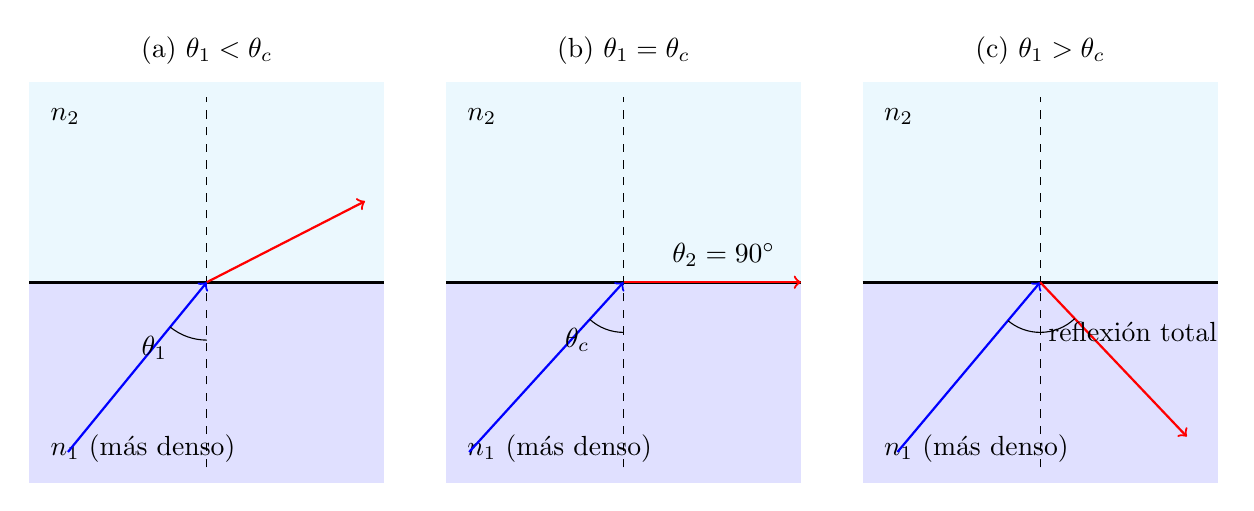
\begin{tikzpicture}[scale=0.98]
  \foreach \s in {0,5.4,10.8}{
    \fill[cyan!8] (\s,0) rectangle +(4.6,2.6);
    \fill[blue!12] (\s,-2.6) rectangle +(4.6,2.6);
    \draw[very thick] (\s,0) -- +(4.6,0);
    \draw[dashed] (\s+2.3,-2.4) -- +(0,4.8);
    \node[anchor=west] at (\s+0.15,2.15) {$n_2$};
    \node[anchor=west] at (\s+0.15,-2.15) {$n_1$ (más denso)};
  }
  \node at (2.3,3.0) {(a) $\theta_1<\theta_c$};
  \node at (7.7,3.0) {(b) $\theta_1=\theta_c$};
  \node at (13.1,3.0) {(c) $\theta_1>\theta_c$};
  \draw[->,blue,thick] (0.5,-2.2) -- (2.3,0);
  \draw[->,red,thick] (2.3,0) -- (4.35,1.05);
  \draw (2.3,-0.75) arc[start angle=-90,end angle=-129.4,radius=0.75];
  \node at (1.62,-0.85) {$\theta_1$};
  \draw[->,blue,thick] (5.7,-2.2) -- (7.7,0);
  \draw[->,red,thick] (7.7,0) -- (10.0,0);
  \draw (7.7,-0.65) arc[start angle=-90,end angle=-132.3,radius=0.65];
  \node at (7.1,-0.75) {$\theta_c$};
  \node at (9.0,0.35) {$\theta_2=90^\circ$};
  \draw[->,blue,thick] (11.25,-2.2) -- (13.1,0);
  \draw[->,red,thick] (13.1,0) -- (15.0,-2.0);
  \draw (13.1,-0.65) arc[start angle=-90,end angle=-130,radius=0.65];
  \draw (13.1,-0.65) arc[start angle=-90,end angle=-46.5,radius=0.65];
  \node at (14.3,-0.65) {reflexión total};
\end{tikzpicture}
\caption{Refracción, ángulo crítico y reflexión interna total.}
\end{figure}

\section{Dispersión}

La \textbf{dispersión} de la luz es la separación de un rayo de luz en sus componentes de color (frecuencias) debido a que cada longitud de onda experimenta un índice de refracción ligeramente distinto en el medio. El ejemplo clásico es un prisma de vidrio: la luz blanca incide y, al refractarse, cada color se desvía un ángulo diferente, produciendo un arcoíris. La luz violeta (menor $\lambda$) se desvía más que la roja (mayor $\lambda$) porque $n(\lambda_{\text{violeta}}) > n(\lambda_{\text{roja}})$.

\begin{figure}[H]
\centering
\begin{tikzpicture}[>=Stealth,scale=1.05]
  \filldraw[fill=cyan!12,draw=black,very thick] (0,-2.3) -- (2.1,2.3) -- (4.2,-2.3) -- cycle;
  \draw[->,very thick] (-3.2,0.3) -- (0.94,0.3);
  \node[above] at (-1.5,0.3) {luz blanca};
  \draw[white,line width=3pt] (0.94,0.3) -- (3.25,-0.2);
  \draw[black!50,thin] (0.94,0.3) -- (3.25,-0.2);
  \foreach \col/\yy/\name in {red/0.45/rojo,orange/0.15/naranja,yellow!80!black/-0.15/amarillo,green!60!black/-0.45/verde,blue/-0.75/azul,violet/-1.05/violeta}{
    \draw[->,\col,very thick] (3.25,-0.2) -- (7.0,\yy);
    \node[\col,anchor=west] at (7.05,\yy) {\name};
  }
\end{tikzpicture}
\caption{Dispersión de la luz blanca al atravesar un prisma.}
\end{figure}

\section{Lentes}

Una \textbf{lente} es un dispositivo óptico transmisor que enfoca o dispersa un haz de luz por medio de la refracción. Las lentes son el componente fundamental de los telescopios refractores y de los oculares. Sus funciones principales en un sistema óptico astronómico son:

\begin{itemize}
    \item Acumular la luz en una pequeña región (concentración).
    \item Producir magnificación de los objetos.
    \item Proveer poder de resolución.
\end{itemize}

\subsection{Tipos de lentes}

\begin{itemize}
    \item \textbf{Lentes convergentes (positivas)}: son más gruesas en el centro que en los bordes. Hacen converger los rayos paralelos en un punto focal real. Ejemplos: biconvexa, plano-convexa, menisco convergente.
    \item \textbf{Lentes divergentes (negativas)}: son más delgadas en el centro. Hacen diverger los rayos paralelos como si provinieran de un punto focal virtual. Ejemplos: bicóncava, plano-cóncava, menisco divergente.
\end{itemize}

\begin{figure}[H]
\centering
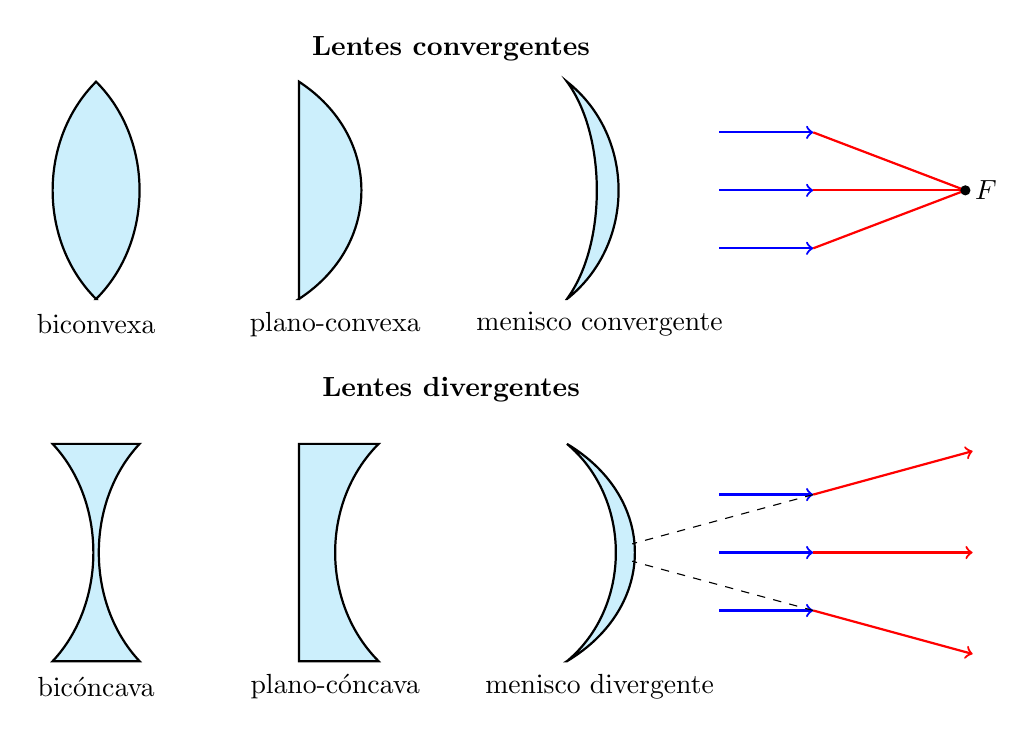
\begin{tikzpicture}[scale=0.92]
  \node[font=\bfseries] at (5.5,3.45) {Lentes convergentes};
  \node[font=\bfseries] at (5.5,-1.25) {Lentes divergentes};
  \filldraw[fill=cyan!20,thick] (0.6,0) .. controls (-0.2,0.8) and (-0.2,2.2) .. (0.6,3)
    .. controls (1.4,2.2) and (1.4,0.8) .. cycle;
  \node at (0.6,-0.35) {biconvexa};
  \filldraw[fill=cyan!20,thick] (3.4,0) -- (3.4,3)
    .. controls (4.55,2.25) and (4.55,0.75) .. cycle;
  \node at (3.9,-0.35) {plano-convexa};
  \filldraw[fill=cyan!20,thick] (7.1,0) .. controls (8.05,0.75) and (8.05,2.25) .. (7.1,3)
    .. controls (7.65,2.25) and (7.65,0.75) .. cycle;
  \node at (7.55,-0.35) {menisco convergente};
  \foreach \y in {0.7,1.5,2.3}{\draw[->,blue,thick] (9.2,\y) -- (10.5,\y);}
  \foreach \y in {0.7,1.5,2.3}{\draw[red,thick] (10.5,\y) -- (12.6,1.5);}
  \fill (12.6,1.5) circle (2pt) node[right] {$F$};
  \begin{scope}[yshift=-5cm]
    \filldraw[fill=cyan!20,thick] (0,0) .. controls (0.75,0.8) and (0.75,2.2) .. (0,3)
      -- (1.2,3) .. controls (0.45,2.2) and (0.45,0.8) .. (1.2,0) -- cycle;
    \node at (0.6,-0.35) {bicóncava};
    \filldraw[fill=cyan!20,thick] (3.4,0) -- (3.4,3) -- (4.5,3)
      .. controls (3.7,2.2) and (3.7,0.8) .. (4.5,0) -- cycle;
    \node at (3.9,-0.35) {plano-cóncava};
    \filldraw[fill=cyan!20,thick] (7.1,0) .. controls (8.0,0.75) and (8.0,2.25) .. (7.1,3)
      .. controls (8.35,2.25) and (8.35,0.75) .. cycle;
    \node at (7.55,-0.35) {menisco divergente};
    \foreach \y in {0.7,1.5,2.3}{\draw[->,blue,thick] (9.2,\y) -- (10.5,\y);}
    \draw[->,red,thick] (10.5,0.7) -- (12.7,0.1);
    \draw[->,red,thick] (10.5,1.5) -- (12.7,1.5);
    \draw[->,red,thick] (10.5,2.3) -- (12.7,2.9);
    \draw[dashed] (10.5,0.7) -- (8.0,1.38);
    \draw[dashed] (10.5,2.3) -- (8.0,1.62);
  \end{scope}
\end{tikzpicture}
\caption{Perfiles de lentes convergentes y divergentes y acción sobre rayos paralelos.}
\end{figure}

\subsection{Formación de imágenes con lentes}

Para una lente delgada convergente de distancia focal $f$, la relación entre la distancia del objeto $d_o$, la distancia de la imagen $d_i$ y la distancia focal está dada por la \textbf{ecuación de la lente delgada}:

$$\frac{1}{f} = \frac{1}{d_o} + \frac{1}{d_i}$$

El \textbf{aumento lateral} es

$$M = -\frac{d_i}{d_o}$$

El signo negativo indica que la imagen está invertida cuando $M<0$.

Para construir la imagen geométricamente se utilizan tres rayos principales:
\begin{enumerate}
    \item Un rayo paralelo al eje óptico que, tras atravesar la lente, pasa por el foco imagen $F'$.
    \item Un rayo que pasa por el centro óptico de la lente sin desviarse.
    \item Un rayo que pasa por el foco objeto $F$ y emerge paralelo al eje óptico.
\end{enumerate}

La intersección de estos rayos determina la posición y el tamaño de la imagen.

\begin{figure}[H]
\centering
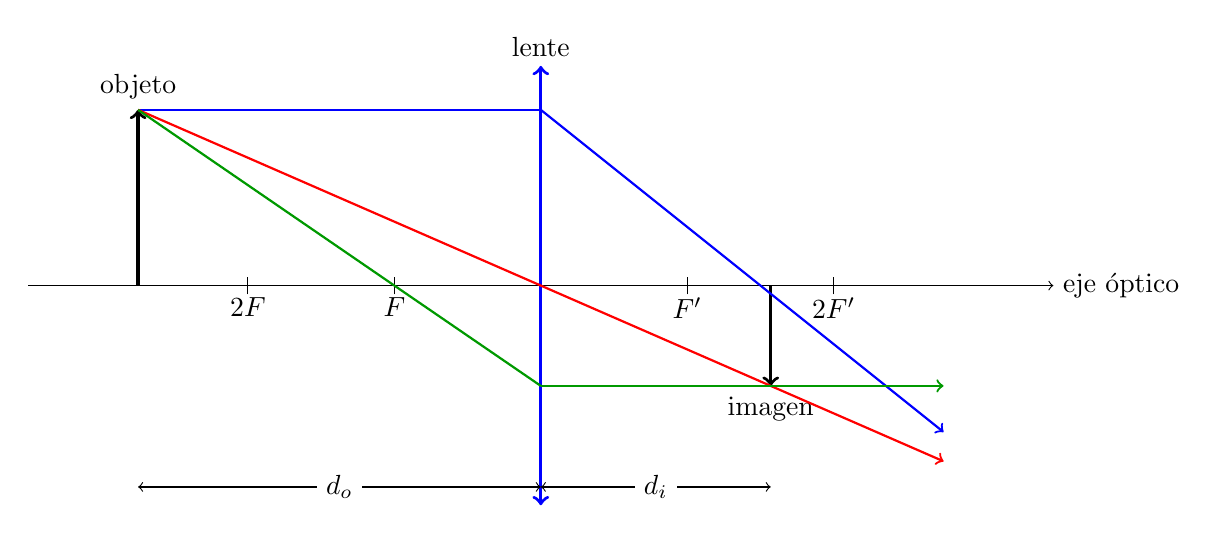
\begin{tikzpicture}[scale=0.93]
  \draw[->] (-7,0) -- (7,0) node[right] {eje óptico};
  \draw[<->,very thick,blue] (0,-3) -- (0,3);
  \node[above] at (0,3) {lente};
  \foreach \x/\lab in {-4/{2F},-2/F,2/{F'},4/{2F'}}{
    \draw (\x,-0.12) -- (\x,0.12) node[below=4pt] {$\lab$};
  }
  \draw[->,very thick] (-5.5,0) -- (-5.5,2.4) node[above] {objeto};
  \draw[->,very thick] (3.14,0) -- (3.14,-1.37) node[below] {imagen};
  \draw[blue,thick] (-5.5,2.4) -- (0,2.4);
  \draw[->,blue,thick] (0,2.4) -- (5.5,-2.0);
  \draw[red,thick,->] (-5.5,2.4) -- (5.5,-2.4);
  \draw[green!60!black,thick] (-5.5,2.4) -- (-2,0) -- (0,-1.37);
  \draw[->,green!60!black,thick] (0,-1.37) -- (5.5,-1.37);
  \draw[<->] (-5.5,-2.75) -- (0,-2.75) node[midway,fill=white] {$d_o$};
  \draw[<->] (0,-2.75) -- (3.14,-2.75) node[midway,fill=white] {$d_i$};
\end{tikzpicture}
\caption{Construcción de una imagen real mediante los tres rayos principales de una lente convergente.}
\end{figure}

\subsection{Aberración cromática en lentes}

La \textbf{aberración cromática} es un tipo de distorsión óptica provocada por la imposibilidad de una lente para enfocar todos los colores (longitudes de onda) en un único punto de convergencia. Dado que el índice de refracción depende de $\lambda$ (dispersión), la distancia focal es ligeramente distinta para cada color: la luz azul se enfoca más cerca de la lente que la luz roja. El resultado es una imagen con bordes coloreados (franjas rojas/azules).

\begin{figure}[H]
\centering
\begin{tikzpicture}[>=Stealth,scale=1.05]
  \draw[->] (-4,0) -- (6.5,0) node[right] {eje óptico};
  \filldraw[fill=cyan!15,draw=blue!60,thick]
    (0,-2.3) .. controls (-0.9,-1.2) and (-0.9,1.2) .. (0,2.3)
    .. controls (0.9,1.2) and (0.9,-1.2) .. cycle;
  \foreach \y in {-1.3,1.3}{
    \draw[black!55,thick] (-3.7,\y) -- (0,\y);
    \draw[blue,very thick] (0,\y) -- (3.0,0);
    \draw[red,very thick] (0,\y) -- (4.6,0);
  }
  \fill[blue] (3,0) circle (2pt);
  \fill[red] (4.6,0) circle (2pt);
  \draw[<->,blue] (0,-1.8) -- (3,-1.8) node[midway,below] {$f_{\text{azul}}$};
  \draw[<->,red] (0,-2.25) -- (4.6,-2.25) node[midway,below] {$f_{\text{rojo}}$};
  \draw[blue,opacity=.35,line width=3pt] (5.6,-0.65) -- (5.6,0.65);
  \draw[red,opacity=.35,line width=3pt] (5.85,-0.65) -- (5.85,0.65);
  \node[align=center] at (5.7,1.25) {bordes\\coloreados};
\end{tikzpicture}
\caption{Aberración cromática: cada longitud de onda posee una distancia focal distinta.}
\end{figure}

\section{Espejos}

Un \textbf{espejo} es una superficie pulida en la que, después de incidir, la luz se refleja siguiendo las leyes de la reflexión. En astronomía, los espejos son el componente principal de los telescopios reflectores, pues colectan luz sin introducir aberración cromática.

\subsection{Tipos de espejos}

\begin{itemize}
    \item \textbf{Espejo plano}: la imagen es virtual, del mismo tamaño y simétrica respecto al plano del espejo.
    \item \textbf{Espejo cóncavo} (convergente): la superficie reflectante es la interior de una casquete esférico. Concentra los rayos paralelos en un foco real.
    \item \textbf{Espejo convexo} (divergente): la superficie reflectante es la exterior. Los rayos paralelos se reflejan divergiendo como si vinieran de un foco virtual detrás del espejo.
\end{itemize}

\begin{figure}[H]
\centering
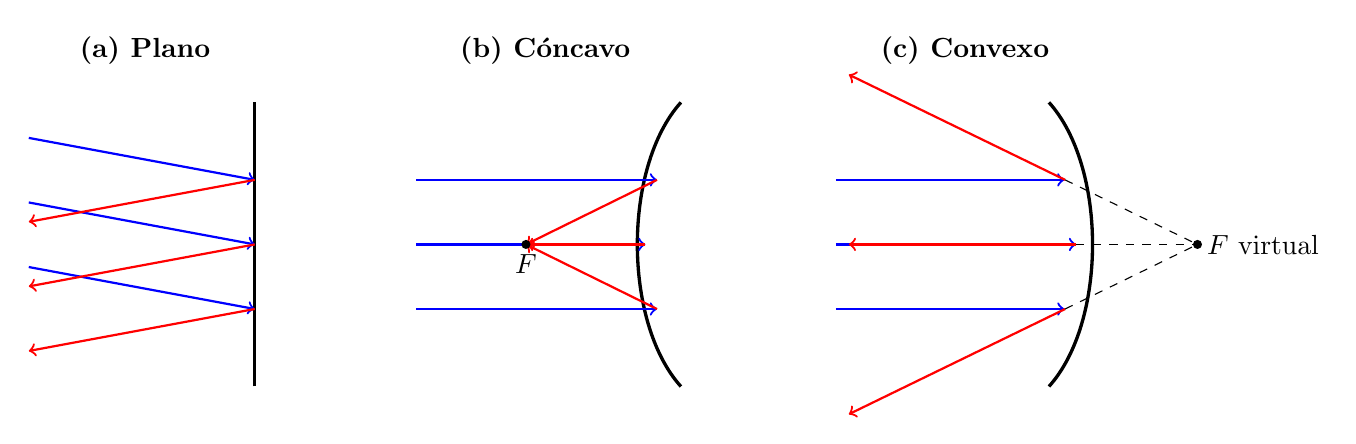
\begin{tikzpicture}[scale=0.82]
  \node[font=\bfseries] at (1.8,3) {(a) Plano};
  \draw[very thick] (3.5,-2.2) -- (3.5,2.2);
  \foreach \y in {-1,0,1}{
    \draw[->,blue,thick] (0,\y+0.65) -- (3.5,\y);
    \draw[->,red,thick] (3.5,\y) -- (0,\y-0.65);
  }
  \begin{scope}[xshift=6cm]
    \node[font=\bfseries] at (2,3) {(b) Cóncavo};
    \draw[very thick] (4.1,-2.2) .. controls (3.2,-1.2) and (3.2,1.2) .. (4.1,2.2);
    \foreach \y in {-1,0,1}{
      \draw[->,blue,thick] (0,\y) -- ({3.55+0.18*abs(\y)},\y);
      \draw[->,red,thick] ({3.55+0.18*abs(\y)},\y) -- (1.7,0);
    }
    \fill (1.7,0) circle (2pt) node[below] {$F$};
  \end{scope}
  \begin{scope}[xshift=12.5cm]
    \node[font=\bfseries] at (2,3) {(c) Convexo};
    \draw[very thick] (3.3,-2.2) .. controls (4.2,-1.2) and (4.2,1.2) .. (3.3,2.2);
    \foreach \y in {-1,0,1}{
      \draw[->,blue,thick] (0,\y) -- ({3.72-0.18*abs(\y)},\y);
    }
    \draw[->,red,thick] (3.55,1) -- (0.2,2.63);
    \draw[->,red,thick] (3.72,0) -- (0.2,0);
    \draw[->,red,thick] (3.55,-1) -- (0.2,-2.63);
    \draw[dashed] (3.55,1) -- (5.6,0);
    \draw[dashed] (3.72,0) -- (5.6,0);
    \draw[dashed] (3.55,-1) -- (5.6,0);
    \fill (5.6,0) circle (2pt) node[right] {$F$ virtual};
  \end{scope}
\end{tikzpicture}
\caption{Espejo plano, cóncavo convergente y convexo divergente.}
\end{figure}

\subsection{Formación de imágenes con espejos esféricos}

Para un espejo esférico de radio de curvatura $R$, la distancia focal es

$$f = \frac{R}{2}$$

y la ecuación del espejo es idéntica en forma a la de la lente delgada:

$$\frac{1}{f} = \frac{1}{d_o} + \frac{1}{d_i}$$

con la convención de signos apropiada (distancias positivas frente al espejo, negativas detrás). El aumento lateral es

$$M = -\frac{d_i}{d_o}$$

Los rayos principales para la construcción geométrica en un espejo cóncavo son:
\begin{enumerate}
    \item Rayo paralelo al eje que se refleja pasando por el foco $F$.
    \item Rayo que pasa por $F$ y se refleja paralelo al eje.
    \item Rayo que pasa por el centro de curvatura $C$ y se refleja sobre sí mismo.
    \item Rayo que incide en el vértice y se refleja simétricamente respecto al eje.
\end{enumerate}

\begin{figure}[H]
\centering
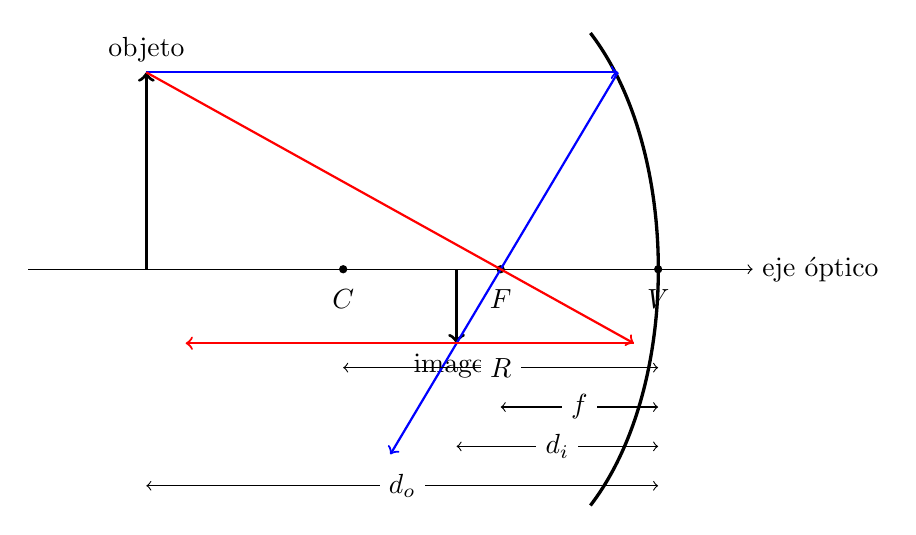
\begin{tikzpicture}[scale=1.0]
  \draw[->] (-8,0) -- (1.2,0) node[right] {eje óptico};
  \draw[very thick] (-0.86,-3) .. controls (0.29,-1.5) and (0.29,1.5) .. (-0.86,3);
  \foreach \x/\lab in {0/V,-2/F,-4/C}{
    \fill (\x,0) circle (1.5pt) node[below=4pt] {$\lab$};
  }
  \draw[->,very thick] (-6.5,0) -- (-6.5,2.5) node[above] {objeto};
  \draw[->,very thick] (-2.56,0) -- (-2.56,-0.94) node[below] {imagen};
  \draw[->,blue,thick] (-6.5,2.5) -- (-0.51,2.5);
  \draw[->,blue,thick] (-0.51,2.5) -- (-3.4,-2.35);
  \draw[->,red,thick] (-6.5,2.5) -- (-2,0) -- (-0.31,-0.94);
  \draw[->,red,thick] (-0.31,-0.94) -- (-6.0,-0.94);
  \draw[<->] (-6.5,-2.75) -- (0,-2.75) node[midway,fill=white] {$d_o$};
  \draw[<->] (-2.56,-2.25) -- (0,-2.25) node[midway,fill=white] {$d_i$};
  \draw[<->] (-2,-1.75) -- (0,-1.75) node[midway,fill=white] {$f$};
  \draw[<->] (-4,-1.25) -- (0,-1.25) node[midway,fill=white] {$R$};
\end{tikzpicture}
\caption{Formación de una imagen real, invertida y reducida en un espejo cóncavo.}
\end{figure}

\subsection{Aberración esférica}

La \textbf{aberración esférica} es un defecto óptico inherente a los espejos (y lentes) de superficie esférica. Los rayos paralelos que inciden cerca del borde del espejo no convergen exactamente en el mismo punto focal que los rayos que inciden cerca del eje óptico. El resultado es una imagen borrosa o con halos.

\begin{figure}[H]
\centering
\begin{tikzpicture}[>=Stealth,scale=1.02]
  \draw[->] (-6.2,0) -- (1.55,0) node[right] {eje óptico};
  \draw[very thick] (-0.94,-3) .. controls (0.31,-1.5) and (0.31,1.5) .. (-0.94,3);
  \node[align=center] at (0.55,2.45) {espejo\\esférico};
  \foreach \y in {-2.2,-1.5,-0.8,0.8,1.5,2.2}{
    \draw[->,blue,thick] (-5.8,\y) -- ({-0.19-0.155*abs(\y)},\y);
  }
  \draw[->,red,thick] (-0.53,2.2) -- (-3.15,0);
  \draw[->,red,thick] (-0.53,-2.2) -- (-3.15,0);
  \draw[->,orange!85!black,thick] (-0.42,1.5) -- (-3.45,0);
  \draw[->,orange!85!black,thick] (-0.42,-1.5) -- (-3.45,0);
  \draw[->,green!55!black,thick] (-0.31,0.8) -- (-3.75,0);
  \draw[->,green!55!black,thick] (-0.31,-0.8) -- (-3.75,0);

  \fill[orange,opacity=.22] (-3.45,0) ellipse (0.48 and 0.22);
  \draw[dashed,red!70] (-3.15,-0.42) -- (-3.15,0.42);
  \draw[dashed,green!60!black] (-3.75,-0.42) -- (-3.75,0.42);
  \fill[red] (-3.15,0) circle (2pt);
  \fill[green!55!black] (-3.75,0) circle (2pt);
  \node[red,fill=white,inner sep=1pt,above right=2pt] at (-3.15,0)
    {$F_m$};
  \node[green!45!black,fill=white,inner sep=1pt,below left=2pt] at (-3.75,0)
    {$F_p$};
  \draw[<->,thick] (-3.75,1.35) -- (-3.15,1.35)
    node[midway,above] {$\Delta f$};
  \node[orange!70!black,fill=white,inner sep=1pt] at (-3.45,-1.25)
    {zona focal extendida};
\end{tikzpicture}
\caption{Aberración esférica: los rayos marginales y paraxiales no comparten un único foco.}
\end{figure}

Este defecto se corrige utilizando espejos con perfil parabólico (que enfocan todos los rayos paralelos en un único punto) o combinaciones de superficies (diseños Cassegrain, Ritchey-Chrétien, etc.), temas que se tratarán al estudiar los telescopios reflectores.